% !TEX root = ../main.tex
\begin{figure*}[t]
\centering
\begin{subfigure}{0.49\linewidth}
  \centering
  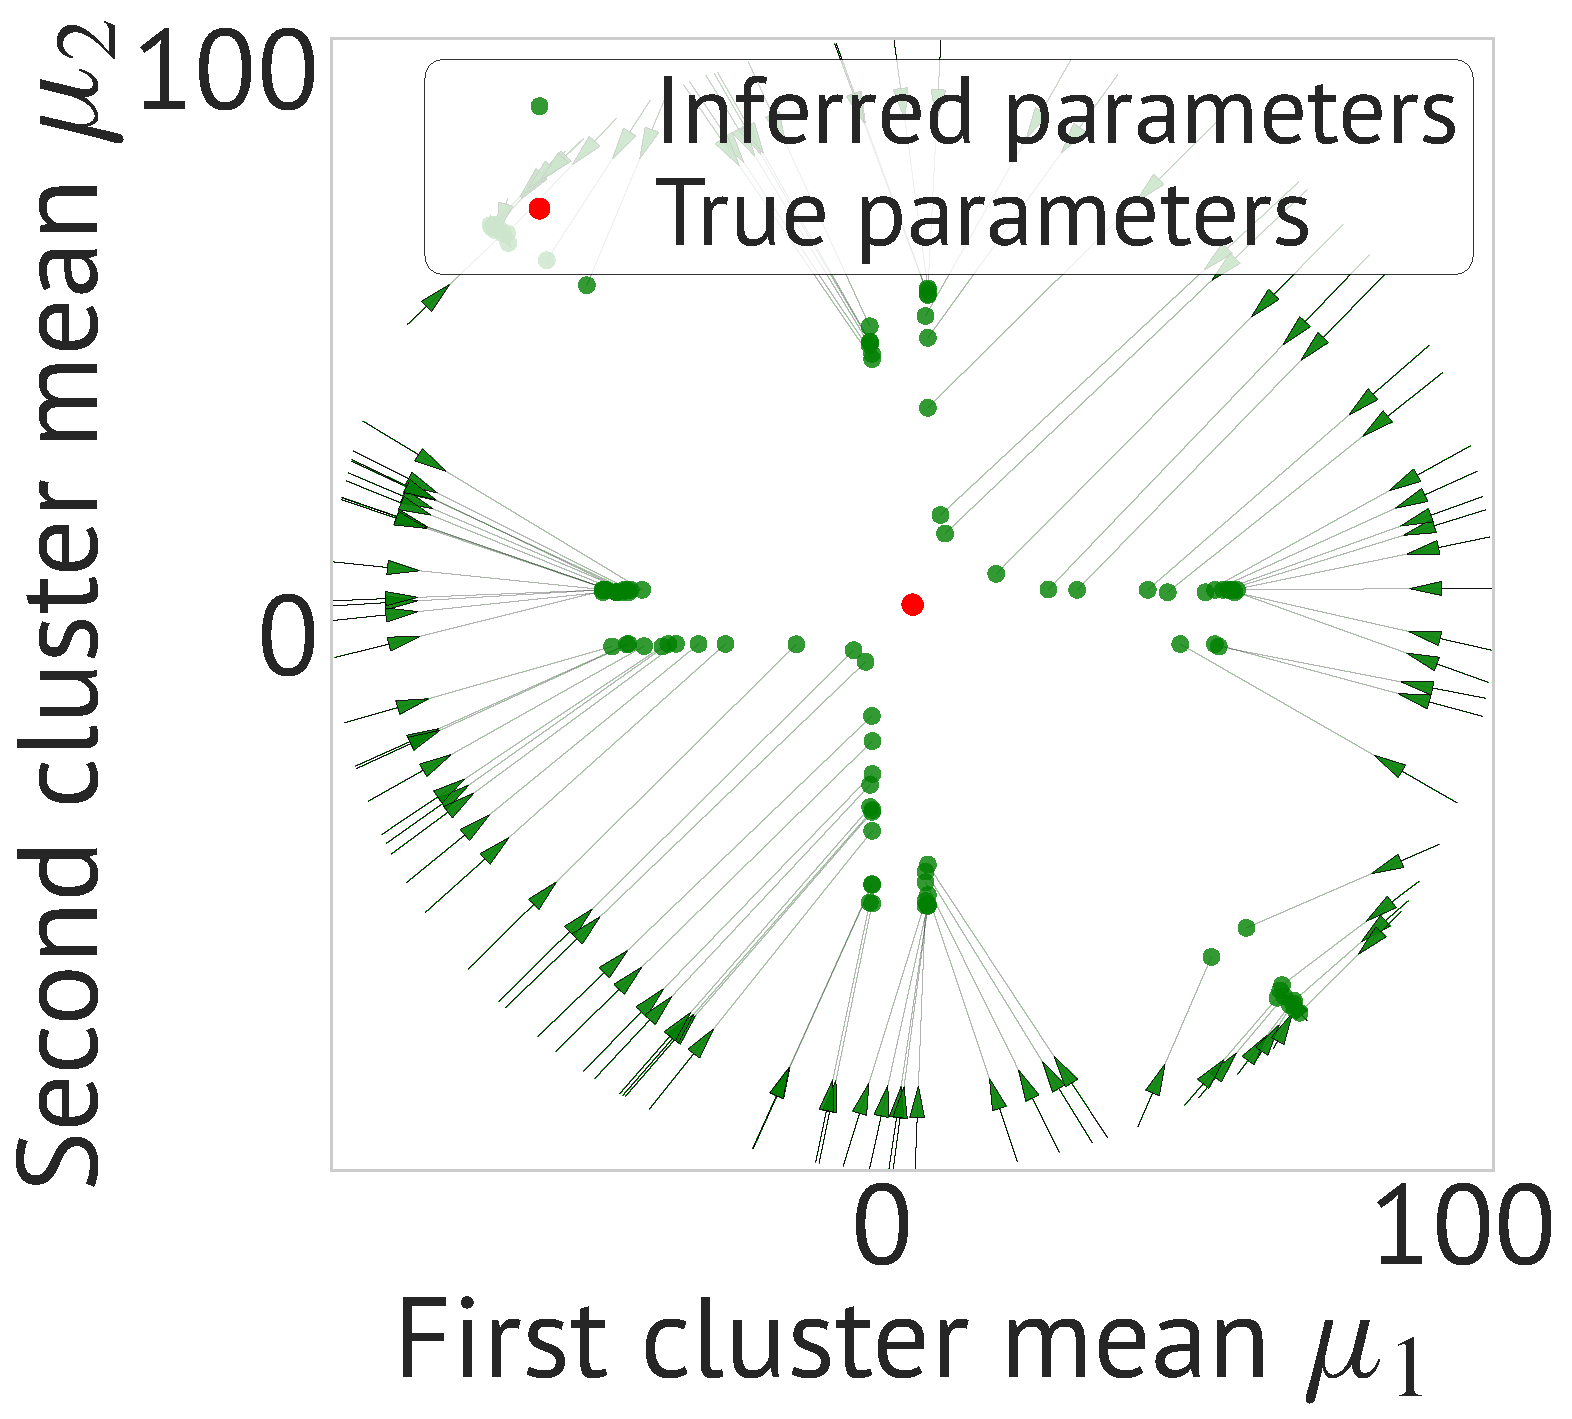
\includegraphics[width=0.8\linewidth]{ch-pvi/img/toy_vanilla}
  \label{fig:bernoulli_vanilla}
  \caption{Variational Inference}
\end{subfigure}
\begin{subfigure}{0.49\linewidth}
    \centering
    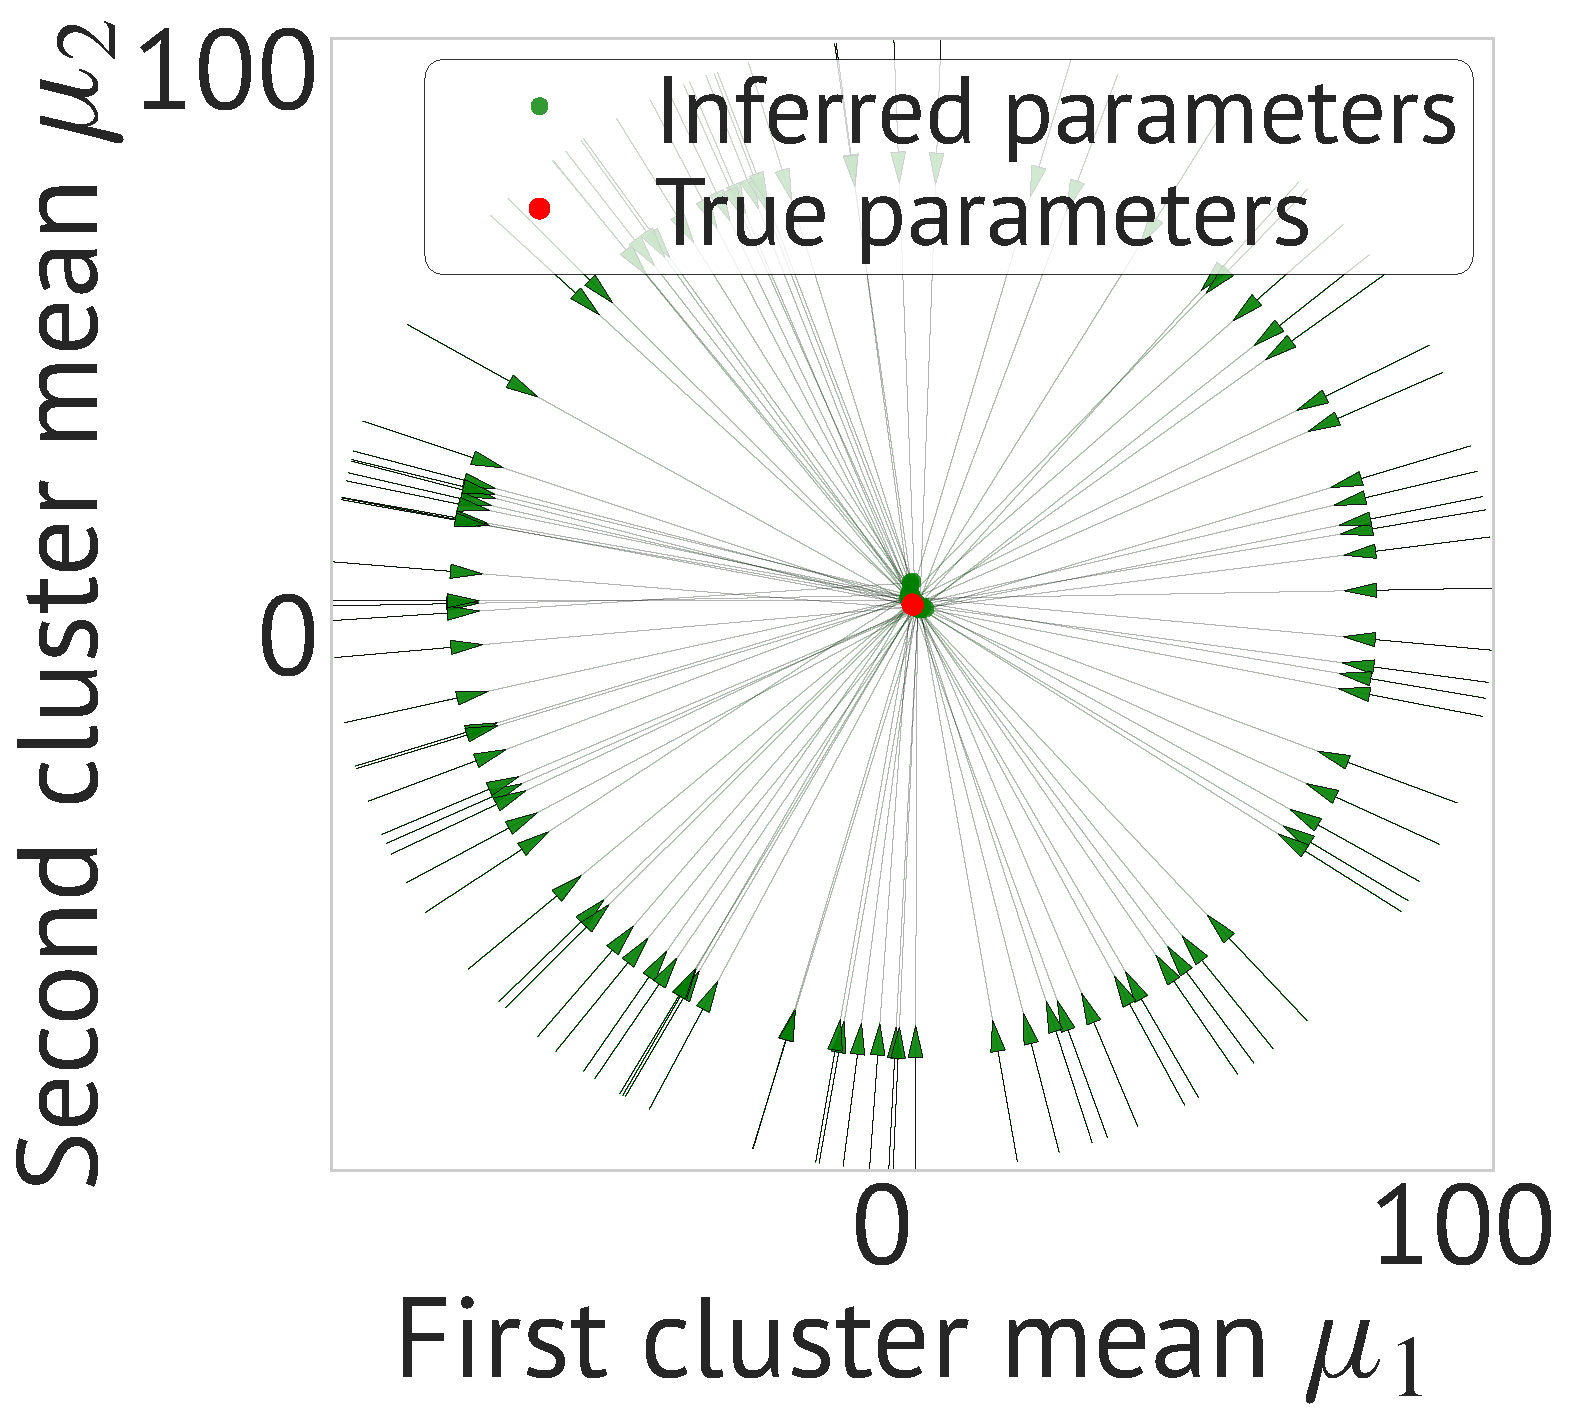
\includegraphics[width=0.8\linewidth]{ch-pvi/img/toy_global}
    \label{fig:bernoulli_global}
    \caption{Proximity \gls{vi}, \Cref{algo:global}}
\end{subfigure}
\caption[\textsc{pvi} makes \textsc{vi} robust to poor initialization]{
\textbf{\Acrlong{PVI} is robust to bad initialization.} We study a Bernoulli factor model. Model parameters are randomly initialized on a ring around the known true parameters (in red) used to generate the data. The arrows start at these parameter initializations and end at the final parameter estimates (shown as green dots). \textbf{(a)} Variational inference with gradient ascent suffers from multiple local optima and cannot reliably recover the truth. \textbf{(b)} \gls{PVI} with an entropy proximity statistic reliably infers the true parameters using \Cref{algo:global}.
}
\label{fig:bernoulli_arrows}
\end{figure*}